\chapter{Instruction Set Architecture}

Processors understand bytes in groups of different sizes. The representation of
this grouping is different on various processors. When we're using this data, we
understand it fully as a group and don't break it up into different parts. We
consider these groups to be \textbf{words} (their term not mine). We would
naturally understand a group of bytes with the most significant byte written to
the left writing the next least significant byte to the right. For instance, a 4
byte word is shown below with the least significant byte being 0-indexed.

\begin{center}
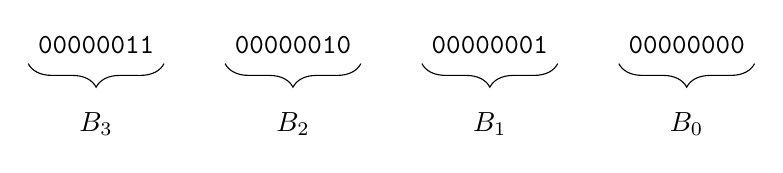
\begin{tikzpicture}
  \node (b3) {\ttfamily 00000011};
  \draw[decorate,decoration={amplitude=3mm,brace,mirror}]
    (b3.south west) -- (b3.south east);
  \node[below of=b3,anchor=center]{$B_3$};

  \node[right of=b3,node distance=2.5cm] (b2) {\ttfamily 00000010};
  \draw[decorate,decoration={amplitude=3mm,brace,mirror}]
    (b2.south west) -- (b2.south east);
  \node[below of=b2,anchor=center]{$B_2$};

  \node[right of=b2,node distance=2.5cm] (b1) {\ttfamily 00000001};
  \draw[decorate,decoration={amplitude=3mm,brace,mirror}]
    (b1.south west) -- (b1.south east);
  \node[below of=b1,anchor=center]{$B_1$};

  \node[right of=b1,node distance=2.5cm] (b0) {\ttfamily 00000000};
  \draw[decorate,decoration={amplitude=3mm,brace,mirror}]
    (b0.south west) -- (b0.south east);
  \node[below of=b0,anchor=center]{$B_0$};
\end{tikzpicture}
\end{center}

\section{ARM}

Currently, the plan is to initially make this secton specifically for ARMv7.

\section{x86\_64}

\begin{listing}[H]
  \inputminted[frame=lines]{asm}{code/hello_world.asm}
  \caption{``Hello world'' program written in x86\_64 assembly for Linux}
  \label{lst:hello-world-asm}
\end{listing}

Assuming the file is called ``\mintinline{console}{hello_world.asm}'' we need to
compile to machine code using \mintinline{console}{nasm -f elf64
  hello_world.asm}. This produces a file named
``\mintinline{console}{hello_world.o}'' which is an object file (more later). To
produce an executable file that will run on the machine use the standard linker:
\mintinline{console}{ld hello_world.o -o hello_world}. This produces an
executable named ``\mintinline{console}{hello_world}''. Running the program
using \mintinline{console}{./hello_world} produces the output
``\mintinline{console}{Hello world!}''.

x86\_64 has 16 general purpose registers: \mintinline{asm}{rax},
\mintinline{asm}{rbx}, \mintinline{asm}{rcx}, \mintinline{asm}{rdx},
\mintinline{asm}{rbp}, \mintinline{asm}{rsi}, \mintinline{asm}{rdi},
\mintinline{asm}{rsp}, \mintinline{asm}{r8}, \mintinline{asm}{r9},
\mintinline{asm}{r10}, \mintinline{asm}{r11}, \mintinline{asm}{r12},
\mintinline{asm}{r13}, \mintinline{asm}{r14}, and \mintinline{asm}{r15}. The
stack pointer is \mintinline{asm}{rsp} and it is always(?) in use.

Note that the system call number goes in register \mintinline{asm}{rax}. Note
that (on x86\_64) the system call number for \mintinline{asm}{write} is
\texttt{1} and for \mintinline{asm}{exit_group} is \texttt{231}. The arguments
to the system call go in registers according to the following table:

{\ttfamily\begin{tabular}{c c}
  \hline
  Index & Register \\
  \hline
  0 & \mintinline{asm}{rdi} \\
  1 & \mintinline{asm}{rsi} \\
  2 & \mintinline{asm}{rdx} \\
  3 & \mintinline{asm}{r10} \\
  4 & \mintinline{asm}{r8} \\
  5 & \mintinline{asm}{r9} \\
\end{tabular}}

In C, \mintinline{asm}{rcx} is used instead of \mintinline{asm}{r10} for the
argument at index 3. The kernel destroys registers in \mintinline{asm}{rcx} and
\mintinline{asm}{r11}. Registers \mintinline{asm}{rbp}, \mintinline{asm}{rbx},
\mintinline{asm}{r12}, \mintinline{asm}{r13}, \mintinline{asm}{r14}, and
\mintinline{asm}{r15} belong to the calling function and are untouched by the
kernel.
